\documentclass{article}
\usepackage[margin=.9in]{geometry}
\usepackage{xcolor}
\usepackage{amsmath}
\usepackage{amssymb}
\usepackage{float}
\usepackage{listings}
\lstset{
  basicstyle=\small\ttfamily,
  breaklines=true,
  frame=single,
  language=python,
  numberstyle=\tiny,
  showstringspaces=false
}
\setlength{\parindent}{0pt}
\setlength{\parskip}{\baselineskip}
\definecolor{mycolor}{rgb}{0.1, 0.1, 0.5}
\title{\textbf{{\huge Transfer Function Design}}}
\author{Christopher Hunt}
\date{}
\usepackage{graphicx} 
\usepackage{fancyhdr}

\begin{document}
\pagestyle{fancy}
\fancyhf{}
\rfoot{ENGR 203}
\lfoot{Christopher Hunt}
\lhead{Transfer Function Design}
\rhead{\thepage}
\maketitle
\section*{\textcolor{mycolor}{Objectives}}
This labs aim is to practice transfer function design using circuit building blocks and to relate a transfer function and circuit response to the analytical solution of the circuit using Laplace transforms. 

For part 1 of the lab a circuit will be designed to realize the transfer function under inspection using only resistors, capacitors and inverting op amps. This circuit design will then be simulated in LTSpice and a Bode plot will be produced. This Bode plot will then be compared to one made from analyzing the s-domain function the circuit was derived from. 

For part 2, the transient function under examination will be converted into the time-domain, this will be plotted and compared to the step response of the simulated circuit. 
\vspace{5mm}
\hrule

\section*{\textcolor{mycolor}{Equipment}}
\begin{itemize}
  \item LTSpice
\end{itemize}
\vspace{5mm}
\hrule

\section*{\textcolor{mycolor}{Transfer Function Analysis}}
The transfer function to be examined is:
\begin{equation}
    F(s) = \frac{200s}{s^2+12s+20}
\end{equation}
To begin we will decompose it and identify it's poles and zeros to construct a Bode plot from this function.
\begin{align*}
    F(s) =& \frac{200s}{s^2+12s+20}\\
    F(s) =& \frac{200s}{(s+10)(s+2)}
\end{align*}
From this we can ascertain these values to help us construct a Bode plot:
$$K = 200 \quad \text{ Simple Zeroes: } n = 1 \quad \text{Poles: } p_1 = 10 \;\; p_2 = 2$$

\begin{figure}[H]
    \centering
    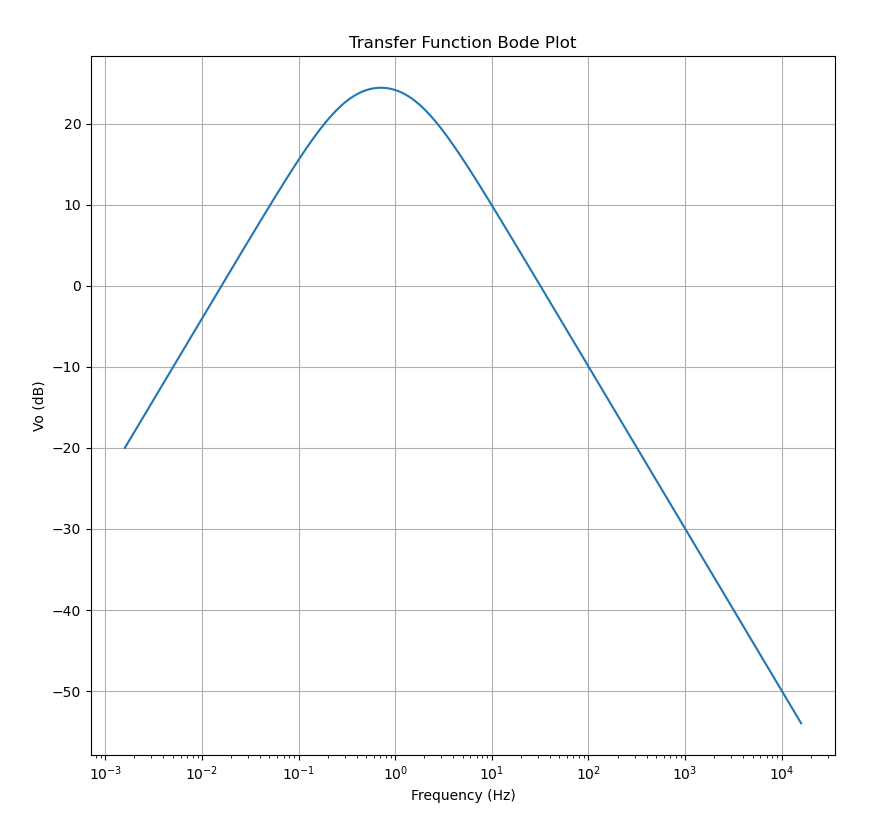
\includegraphics[width=1\textwidth]{png/trans_bode.png}
    \caption{Transfer Function Bode Plot}
    \label{fig:Transfer Function Bode Plot}
\end{figure}
From this function we can isolate the max $V_o$ and $\omega_o$ of the circuit.
$$\text{Max }V_o = 24.44\;dB\qquad \omega_o = 0.71 Hz$$


\section*{\textcolor{mycolor}{Circuit Construction}}
This transfer function can be decomposed in such a way that will allow us to construct a potential circuit that will output this transfer function. F(s) can be decomposed as follows:
\begin{align*}
    F(s) =& \frac{200s}{(s+10)(s+2)}\\
    F(s) =& \frac{s}{s+10}+\frac{1}{s+2}+200
\end{align*}
From inspection, this transfer function can be constructed using a CR-circuit for the first term, an RC-circuit for the second term, and two inverting
op amps for the third. The design and component values can be viewed in figure 2.
\begin{figure}[H]
    \centering
    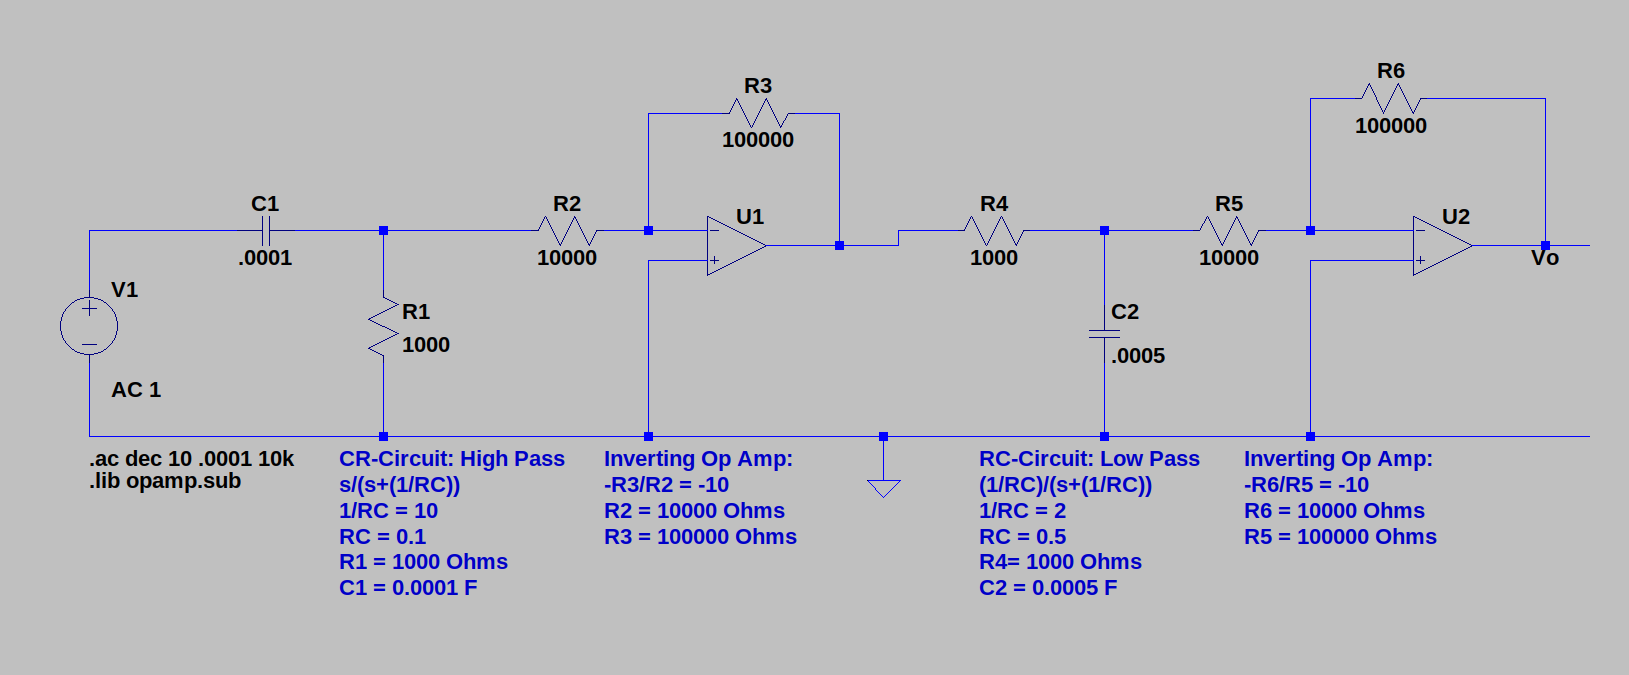
\includegraphics[width=1\textwidth]{png/const_circ_diagram.png}
    \caption{Constructed Circuit}
    \label{fig:Constructed Circuit}
\end{figure}
Running the LTSpice simulation of this circuit, taking data from Vo node, we see the corresponding Bode plot (fig. 3).
\begin{figure}[H]
    \centering
    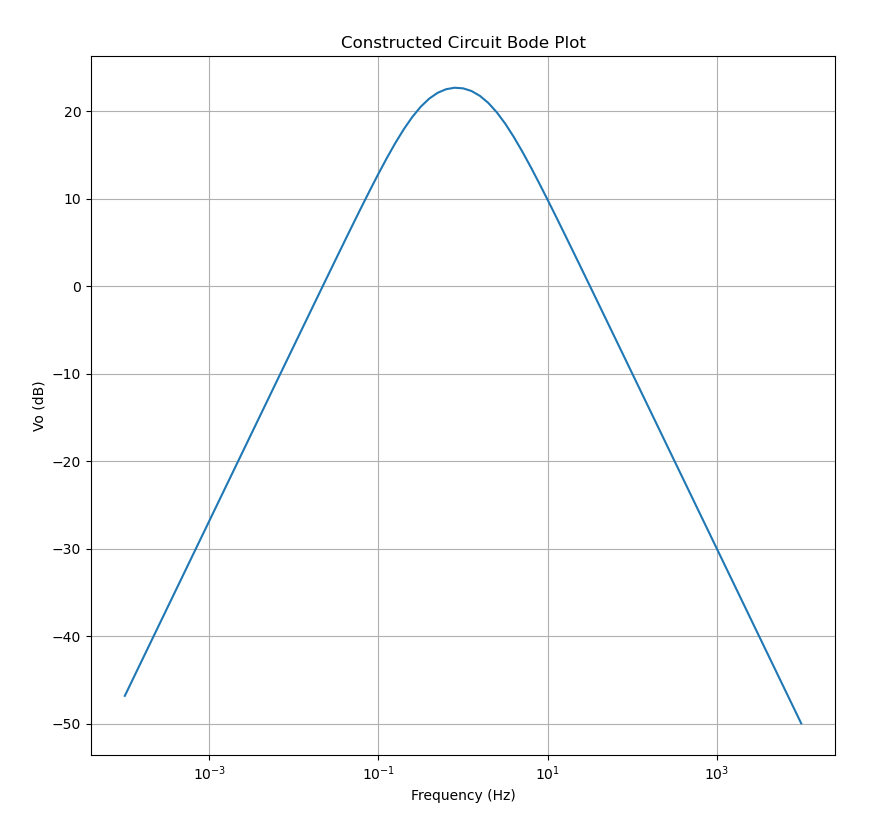
\includegraphics[width=1\textwidth]{png/const_bode.png}
    \caption{Bode Plot for Constructed Circuit}
    \label{fig:Bode Constructed Circuit}
\end{figure}
From this data we can isolate the max $V_o$ and $\omega_o$ of the circuit.
$$\text{Max }V_o = 23.61\;dB\qquad \omega_o = 0.79 Hz$$

\section*{\textcolor{mycolor}{Transient Response Analysis}}
\subsection*{\textcolor{mycolor}{Theoretical Analyses}}
From the given transfer function (eq. 1) we can perform an Inverse Laplace Transform to acquire the corresponding time-domain function. To do this we will decompose F(s) using the method of residuals.
\begin{equation*}
    \frac{200s}{s^2+12s+20} = \frac{A}{s+10} + \frac{B}{s+2}
\end{equation*}
\begin{align*}
    A=(s+10)F(s)|_{s=-10}=& \frac{200(-10)}{-10+2} = 250\\
    B=(s+2)F(s)|_{s=-2}=& \frac{200(-2)}{-2+10} = -50\\
\end{align*}
\begin{equation*}
    \frac{200s}{s^2+12s+20} = \frac{250}{s+10} - \frac{50}{s+2}
\end{equation*}
\\
From this we can use an inverse Laplace Transform table to find the corresponding time-domain functions.
\begin{equation*}
    \mathcal{L}^{-1}\{F(s)\}=250e^{-10t}-50e^{-2t}
\end{equation*}

\begin{figure}[H]
    \centering
    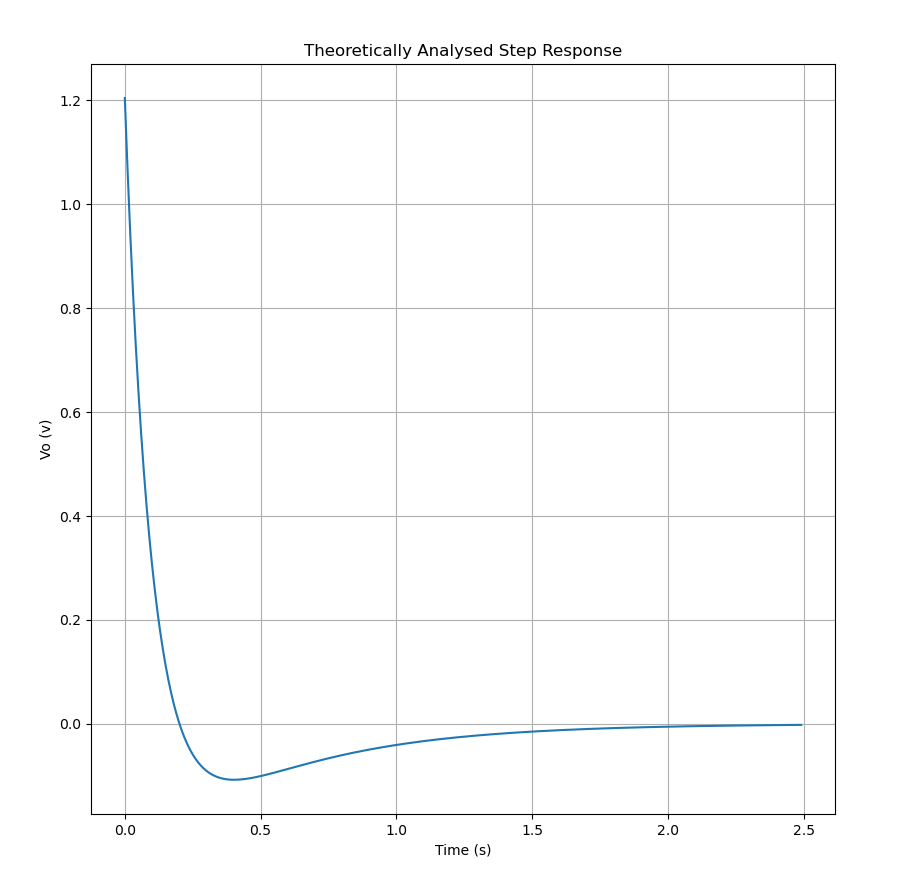
\includegraphics[width=1\textwidth]{png/theoretic_step_resp.png}
    \caption{Theoretically Analysed Step Response}
    \label{fig:Theoretically Analysed Step Response}
\end{figure}

\subsection*{\textcolor{mycolor}{Simulated Analyses}}
By initiating a step response using LTSpice, we were able to simulate the constructed circuits step response (fig. 4). 
\begin{figure}[H]
    \centering
    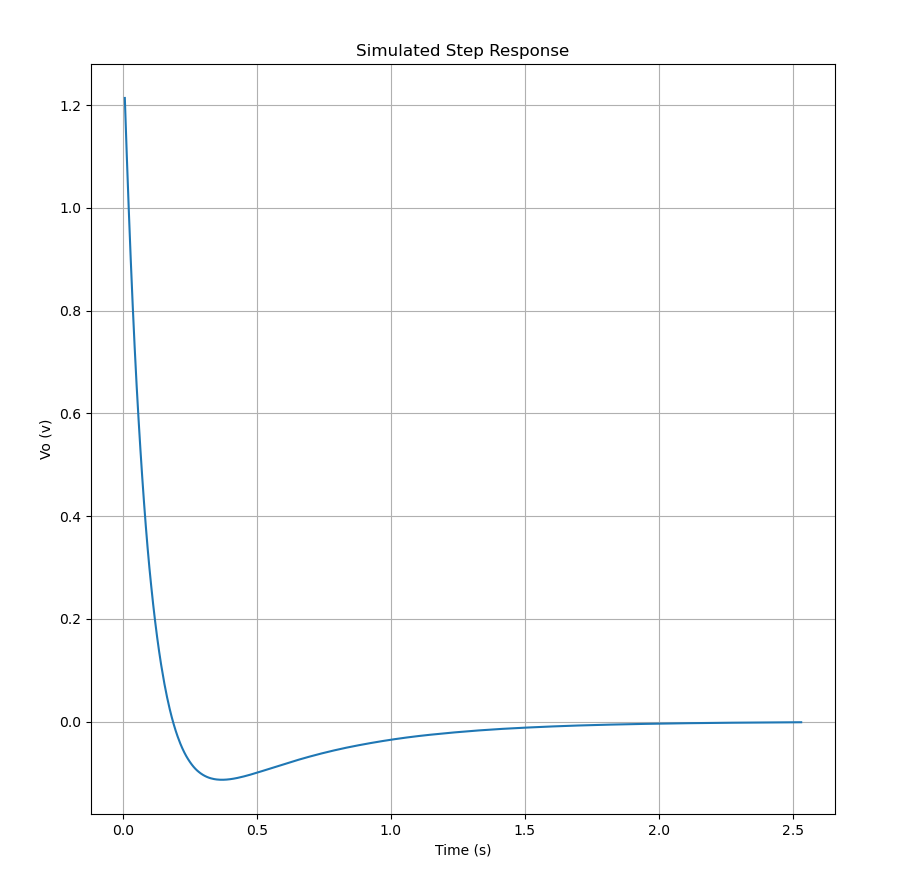
\includegraphics[width=1\textwidth]{png/sim_step_resp.png}
    \caption{Simulated Step Response}
    \label{fig:Simulated Step Response}
\end{figure}
\vspace{5mm}
\hrule

\section*{\textcolor{mycolor}{Conclusion}}
This lab aimed to practice transfer function design using circuit building blocks and relate the transfer function and circuit response to the analytical solution of the circuit using Laplace transforms. First, the transfer function was decomposed to identify its poles and zeros and construct a Bode plot. 

The Bode plot revealed the maximum output voltage ($V_o$) of 24.44 dB and the corresponding angular frequency ($\omega_o$) of 0.71 Hz. Next, a circuit was designed to realize the transfer function using resistors, capacitors, and inverting op amps. The designed circuit was simulated in LTSpice, and a Bode plot was generated. 

The simulated Bode plot showed a maximum $V_o$ of 23.61 dB and $\omega_o$ of 0.79 Hz. Additionally, the theoretical analysis involved performing an inverse Laplace transform on the transfer function to obtain the corresponding time-domain function. The step response of the circuit was theoretically analyzed, resulting in the time-domain function of $250e^{-10t} - 50e^{-2t}$.

The constructed circuit was also simulated in LTSpice to obtain the step response. The simulated step response closely matched the theoretically analyzed response.

In conclusion, the lab successfully demonstrated the process of transfer function design, circuit simulation, and comparison of theoretical and simulated responses. The designed circuit closely approximated the desired transfer function, indicating the effectiveness of the design approach.

\newpage

\section*{\textcolor{mycolor}{Appendix}}
\begin{lstlisting}
# Christopher Hunt
# 5/1/2023
# const_circuit_analysis.py
import numpy as np
import matplotlib.pyplot as plt

def transfer_func(s):
    max_val = None

    for i, val in enumerate(s):
        val_db = 20 * np.log10(np.abs((val * 200) / ((val + 10) * (val + 2))))

        if max_val is None or val_db > max_val:
            max_val = val_db
            max_freq_index = i

        s[i] = val_db

    return s, max_val, max_freq_index

def extract_data(data_string):
    data_lines = data_string.strip().split('\n')
    x = []
    y = []

    for line in data_lines:
        freq, value = line.split()
        freq = float(freq)
        value = float(value.split(",")[0].replace('dB','').replace('(',''))
        x.append(freq)
        y.append(value)

    return x, y

filename = 'ENGR203_lab3.txt'  # Replace with your actual filename

with open(filename, 'r', encoding='utf-8') as file:
    data_string = file.read()

freq, v_out1 = extract_data(data_string)

# Transfer Function values
values = np.arange(0.01, 100000.01, 0.05).tolist()
s = [1j * val for val in values]

v_out2, max_val, max_freq_index = transfer_func(s)
hertz = [val / (2 * np.pi) for val in values]

print("Transfer Function Bode Plot:")
print(f"Max Vo: {max_val} dB")
print(f"Frequency: {hertz[max_freq_index]} Hz")
print()

print("Constructed Circuit Bode Plot:")
print(f"Max Vo: {max(v_out1)} dB")
print(f"Frequency: {freq[v_out1.index(max(v_out1))]} Hz")
print()

fig, axs = plt.subplots(1, 2, figsize=(15, 5))

axs[0].semilogx(hertz, v_out2)
axs[0].grid(True)
axs[0].set_xlabel('Frequency (Hz)')
axs[0].set_ylabel('Vo (dB)')
axs[0].set_title('Transfer Function Bode Plot')

axs[1].semilogx(freq, v_out1)
axs[1].grid(True)
axs[1].set_xlabel('Frequency (Hz)')
axs[1].set_ylabel('Vo (dB)')
axs[1].set_title('Constructed Circuit Bode Plot')

plt.tight_layout()
plt.show()

\end{lstlisting}


\begin{lstlisting}
# Christopher Hunt
# 5/1/2023
# step_response_analysis.py
import numpy as np
import matplotlib.pyplot as plt

def extract_data(data_string):
    data_lines = data_string.strip().split('\n')
    x = []
    y = []

    for line in data_lines:
        freq, value = line.split()
        freq = float(freq)
        value = float(value)
        x.append(freq)
        y.append(value)

    return x, y

def time_domain(t):
    sf = 1/166 # scaling factor
    output = [sf*(250*np.exp(-10*time)-50*np.exp(-2*time)) for time in t]
    return output

# Extract LTSpice Data
filename = "./ENGR203_lab3_step_response.txt"
with open(filename, 'r', encoding='utf-8') as file:
    data_string = file.read()

time_1, v_out_1 = extract_data(data_string)

# Inverse Laplace Transform
time_2 = np.arange(0, 2.5, 0.01).tolist()
v_out_2 = time_domain(time_2)


plt.plot(time_2, v_out_2)
plt.grid(True)
plt.xlabel('Time (s)')
plt.ylabel('Vo (v)')
plt.title('Theoretically Analysed Step Response')
plt.show()

plt.plot(time_1, v_out_1)
plt.grid(True)
plt.xlabel('Time (s)')
plt.ylabel('Vo (v)')
plt.title('Simulated Step Response')
plt.show()
\end{lstlisting}
\end{document}